\documentclass[letterpaper,12pt,fleqn]{article}
\usepackage{matharticle}
\usepackage{siunitx}
\pagestyle{plain}
\begin{document}

\begin{center}
\Large Math-1003b Homework \#8 Solutions
\end{center}

\vspace{0.5in}

\underline{Reading}

\bigskip

\begin{itemize}
\item Section 9.2 and 9.3
\end{itemize}

\bigskip

\underline{Problems}

\bigskip

\begin{enumerate}
\item Determine the domain for the following function:
  \[f(x)=\sqrt{-\frac{(x+5)(4-x)^2}{x(1-x)(x-2)^2}}\]
  Express the domain in interval notation.

  A negative value under the square root is not allowed, so we turn this into
  an inequality problem - the value under the square root must be nonnegative,
  in other words, greater than or equal to 0:
  \[-\frac{(x+5)(4-x)^2}{x(1-x)(x-2)^2}\ge0\]
  Everything is already factored, so let's take care of ``backwards'' factors
  by factoring out (-1) - remember that everything within the parens must
  change sign! Let's start with $(4-x)^2$:
  \[(4-x)^2=[-(x-4)]^2=(-1)^2(x-4)^2=(1)(x-4)^2=(x-4)^2\]
  So the even exponent gets rid of the (-1) that we factored out. So we now
  have:
  \[-\frac{(x+5)(x-4)^2}{x(1-x)(x-2)^2}\ge0\]
  Now, let's take care of the $(1-x)$:
  \[(1-x)=-(x-1)\]
  Note that the this (-1) will cancel out the leading negative and we are left
  with:
  \[\frac{(x+5)(x-4)^2}{x(x-1)(x-2)^2}\ge0\]
  Thus, we have zeros at $x=-5,4$ and poles at $x=0,1,2$. Let's graph those
  first:

  \bigskip

  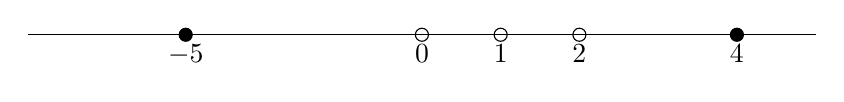
\begin{tikzpicture}
    \draw (-5,0) -- (5,0);
    \node [circle,draw,fill,scale=0.5] (a) at (-3,0) {};
    \node [below] at (a) {$-5$};
    \node [circle,draw,scale=0.5] (b) at (0,0) {};
    \node [below] at (b) {$0$};
    \node [circle,draw,scale=0.5] (c) at (1,0) {};
    \node [below] at (c) {$1$};
    \node [circle,draw,scale=0.5] (d) at (2,0) {};
    \node [below] at (d) {$2$};
    \node [circle,draw,fill,scale=0.5] (e) at (4,0) {};
    \node [below] at (e) {$4$};
  \end{tikzpicture}

  Note that we allow equality so the zeros are included; however, poles are
  never included.

  Next, build a test point table. Remember that the expression can only change
  sign when crossing a zero or a pole, so pick a test point in each on the 6
  intervals to see what the sign is in that interval:

  \begin{tabular}{c|ccccc|c}
    & $x+5$ & $(x-4)^2$ & $x$ & $x-1$ & $(x-2)^2$ & \\
    \hline
    $-6$ & $-$ & $+$ & $-$ & $-$ & $+$ & $-$ \\
    $-1$ & $+$ & $+$ & $-$ & $-$ & $+$ & $+$ \\
    $\frac{1}{2}$ & $+$ & $+$ & $+$ & $-$ & $+$ & $-$ \\
    $1\frac{1}{2}$ & $+$ & $+$ & $+$ & $+$ & $+$ & $+$ \\
    $3$ & $+$ & $+$ & $+$ & $+$ & $+$ & $+$ \\
    $5$ & $+$ & $+$ & $+$ & $+$ & $+$ & $+$
  \end{tabular}

  Now, since we want $\ge0$, we want the positive intervals:

  \bigskip

  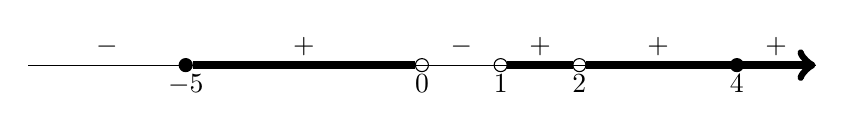
\begin{tikzpicture}
    \draw (-5,0) -- (5,0);
    \node [circle,draw,fill,scale=0.5] (a) at (-3,0) {};
    \node [below] at (a) {$-5$};
    \node [circle,draw,scale=0.5] (b) at (0,0) {};
    \node [below] at (b) {$0$};
    \node [circle,draw,scale=0.5] (c) at (1,0) {};
    \node [below] at (c) {$1$};
    \node [circle,draw,scale=0.5] (d) at (2,0) {};
    \node [below] at (d) {$2$};
    \node [circle,draw,fill,scale=0.5] (e) at (4,0) {};
    \node [below] at (e) {$4$};
    \node [above] at (-4,0) {$-$};
    \node [above] at (-1.5,0) {$+$};
    \node [above] at (0.5,0) {$-$};
    \node [above] at (1.5,0) {$+$};
    \node [above] at (3,0) {$+$};
    \node [above] at (4.5,0) {$+$};
    \draw [line width=1mm] (a) to (b);
    \draw [line width=1mm] (c) to (d);
    \draw [line width=1mm] (d) to (e);
    \draw [line width=1mm,->] (d) to (5,0);
  \end{tikzpicture}

  Note that there is even multiplicity at $x=2,4$, so we do not change sign
  at these points.

  Finally, construct the interval notation as a union of the positive
  intervals. Note that we need to honor the holes at $x=1,2$ but the endpoint
  at $x=4$ gets swallowed up into the ray:
  \[x\in[-5,0)\cup(1,2)\cup(2,\infty)\]

\item Solve the following inequality, expressing the answer in interval
  notation:
  \[x^2+4x\ge 21\]

  First, we need to make sure that we are comparing against $0$;
  \[x^2+4x-21\ge0\]
  Now factor:
  \[(x+7)(x-3)\ge0\]
  So we have zeros at $x=-7,3$. Using the same techniques as in problem 1
  we get:

  \bigskip

  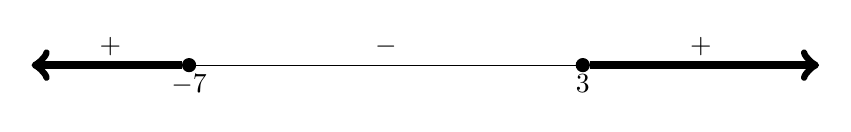
\begin{tikzpicture}
    \draw (-5,0) -- (5,0);
    \node [draw,circle,fill,scale=0.5] (a) at (-3,0) {};
    \node [below] at (a) {$-7$};
    \node [draw,circle,fill,scale=0.5] (b) at (2,0) {};
    \node [below] at (b) {$3$};
    \node [above] at (-4,0) {$+$};
    \node [above] at (-0.5,0) {$-$};
    \node [above] at (3.5,0) {$+$};
    \draw [line width=1mm,<-] (-5,0) to (a);
    \draw [line width=1mm,->] (b) to (5,0);
  \end{tikzpicture}

  $x\in(-\infty,-7]\cup[3,\infty)$
  
  Now state the answer (don't do any additional work) for the following in
  interval notation:
  \[x^2+4x-21<0\]

  This is just the complement of the previous solution:

  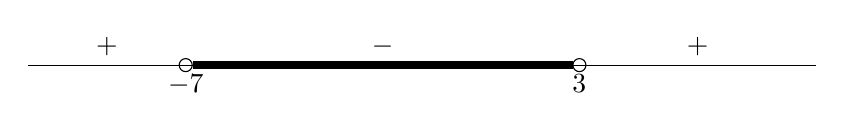
\begin{tikzpicture}
    \draw (-5,0) -- (5,0);
    \node [draw,circle,scale=0.5] (a) at (-3,0) {};
    \node [below] at (a) {$-7$};
    \node [draw,circle,scale=0.5] (b) at (2,0) {};
    \node [below] at (b) {$3$};
    \node [above] at (-4,0) {$+$};
    \node [above] at (-0.5,0) {$-$};
    \node [above] at (3.5,0) {$+$};
    \draw [line width=1mm] (a) to (b);
  \end{tikzpicture}

  $x\in(-7,3)$
  
\item Solve for $x$ (Hint: what kind of equation does this look like?):
  \[(x+1)^2+3\abs{x+1}-4=0\]

  Note that $\abs{x+1}^2=\abs{(x+1)^2}=(x+1)^2$ since something squared is
  always nonnegative. Thus, we can rewrite the above as follows:
  \[\abs{x+1}^2+3\abs{x+1}-4=0\]
  So this is just a quadratic in $\abs{x+1}$ instead of just $x$. So factor it:
  \[(\abs{x+1}+4)(\abs{x+1}-1)=0\]
  Thus, $\abs{x+1}+4=0$ or $\abs{x+1}-1=0$. Start with the first case:
  \[\abs{x+1}=-4\]
  We don't have to go any farther with this case since an absolute value can
  never be negative. So let's look at the second case:
  \[\abs{x+1}=1\]
  When we remove the absolute value we need to compensate with a plus/minus.
  Normally, the plus/minus goes on the side with the absolute value, but a
  short cut with equations only (not inequalities!) allows us to place the
  plus/minus on the other side for convenience:
  \[x+1=\pm1\]
  This results in two cases:

  \bigskip

  \begin{minipage}{2in}
    $x+1=1$ \\
    $x=0$
  \end{minipage}
  \begin{minipage}{2in}
    $x+1=-1$ \\
    $x=-2$
  \end{minipage}

  \bigskip

  Indeed, plugging these two values in to the original equations shows that
  these are the solutions:
  \[x=0,-2\]

\item Smallville, USA has designed their downtown so that their city hall,
  fire station, and police station all occur on a line. If the fire station
  is at the point 0 on the line and the police station is at the point 3 on
  the line, and city hall is twice as far from the fire station as the police
  station, then can you tell exactly where city hall is on the line? You must
  explain exactly how you determine this.

  The purpose of this problem is to show the connection between absolute value
  and distance. Let $x$ be the position of city hall. This means that:

  $\abs{x-0}=\abs{x}=$ distance between city hall and fire station

  $\abs{x-3}=$ distance between city hall and police station

  Since the distance from city hall to the fire station is twice as far as the
  distance between city hall and the police station, we have:
  \[\abs{x}=2\abs{x-3}\]
  Solving this, we have:
  \[x=\pm2(x-3)\]
  This gives rise to two cases:

  \bigskip

  \begin{minipage}{2in}
    $x=2(x-3)$ \\
    $x=2x-6$ \\
    $x=6$
  \end{minipage}
  \begin{minipage}{2in}
    $x=-2(x-3)$ \\
    $x=-2x+6$ \\
    $3x=6$ \\
    $x=2$
  \end{minipage}

  \bigskip

  So there are two possible positions for city hall $x=2$ or $x=6$. Note that
  when $x=2$ the distance between the fire department and city hall is $2$
  and between the police department and city hall is $1$. For $x=6$, the
  distances are $6$ and $3$. In both cases the distance from city hall to the
  fire station is twice the distance from city hall to the police station.

  Therefore, we cannot tell for sure where city hall is located from the given
  information.
\end{enumerate}

\end{document}
